\documentclass{article}
% if you need to pass options to natbib, use, e.g.:
    % \PassOptionsToPackage{numbers, compress}{natbib}
% before loading project
% ready for submission
\usepackage[preprint]{zsupport/project}
% to avoid loading the natbib package, add option nonatbib:
%    \usepackage[nonatbib]{project}

% https://www.overleaf.com/read/wzwnrbbwrvyx
% https://tex.stackexchange.com/questions/162207/algorithm2e-comment-style
% https://tex.stackexchange.com/questions/298339/how-to-insert-a-continue-in-while-command-of-algorithm2e
% https://tex.stackexchange.com/questions/195991/aligning-in-and-out-text-for-algorithms
% https://tex.stackexchange.com/questions/155542/algorithm-write-if-then-return-or-else-return-in-one-line
\usepackage[linesnumbered,ruled,vlined]{algorithm2e}

% https://tex.stackexchange.com/questions/200730/how-to-have-the-algorithmicx-comment-symbol-in-algorithm2e
\SetKwComment{Comment}{$\triangleright$\ }{}
% \newcommand\mycommfont[1]{\footnotesize\ttfamily\textcolor{black}{#1}}
% \SetCommentSty{mycommfont}

\SetKwInput{KwInput}{Input}                % Set the Input
\SetKwInput{KwOutput}{Output}              % set the Output

\SetKw{Andd}{and} % `\And` already exists
\SetKw{Break}{break}
\SetKw{Continue}{continue}
\SetKw{Return}{return}

% https://english.stackexchange.com/questions/338/when-is-l-doubled

% \newcommand{\all}{\textbf{all}~}

\newcommand{\both}{\textbf{both}~}
    \newcommand{\andd}{\textbf{and}~}

\newcommand{\butalso}{\textbf{but also~}}
    \newcommand{\notonly}{\textbf{not only~}}

\newcommand{\cf}{cf.~}

\newcommand{\eg}{e.g.~}
\newcommand{\either}{\textbf{either~}}
    \newcommand{\orr}{\textbf{or}~}
% \newcommand{\every}{\textbf{every~}}

\newcommand{\first}{\textbf{Firstly},~}
    \newcommand{\second}{\textbf{Secondly},~}
    \newcommand{\third}{\textbf{Third},~}
    \newcommand{\fourth}{\textbf{Fourth},~}
    \newcommand{\final}{\textbf{Finally},~}
    \newcommand{\last}{\textbf{Lastly},~}

% \newcommand{\from}{\textbf{from}~}
%     \newcommand{\tob}{\textbf{to}~}

% \newcommand{\never}{\textbf{never}~}
% \newcommand{\no}{\textbf{no}}
\newcommand{\nott}{\textbf{not}~}

\newcommand{\ie}{i.e.~}
\newcommand{\incl}{incl.~} % https://dictionary.cambridge.org/dictionary/english/incl
\newcommand{\iiddot}{i.i.d}
% \newcommand{\iid}{\iiddot~} % many tildes may cause compile error, eg in `~\iid`
\newcommand{\st}{s.t.~}
\newcommand{\vs}{vs.~}

\newcommand{\orrr}{\textbf{or}~}

\newcommand{\wrt}{with respect to~}

% https://tex.stackexchange.com/questions/57152/how-to-draw-graphs-in-latex
% https://tex.stackexchange.com/questions/300098/draw-a-node-as-a-square-with-tikz
% https://tex.stackexchange.com/questions/350049/tikz-pgfplots-how-to-make-tikzpcture-fit-the-parent-figure-subfigure-float-envi/
% https://rmwu.github.io/tutorial/latex/2019/11/21/positioning/
% https://texample.net/tikz/examples/
\usepackage{tikz}
\usetikzlibrary{positioning, shapes.geometric, backgrounds}
% \usetikzlibrary{positioning, shapes, shadows, arrows}

% https://tex.stackexchange.com/questions/5461/is-it-possible-to-change-the-size-of-an-arrowhead-in-tikz-pgf/161238#161238
% https://tex.stackexchange.com/questions/409881/self-loop-arrowhead-different-cannot-change
% https://github.com/pgf-tikz/pgf/issues/1008
    % [>={Arrowtype}] this means "make all arrows {ArrowType}" and you supply this to generic style settings.
    % [-{Arrowtype}] this means "put an end arrow head {ArrowType}" and you supply this style to paths and edges
\usetikzlibrary{arrows.meta}

% https://tex.stackexchange.com/questions/13625/subcaption-vs-subfig-best-package-for-referencing-a-subfigure
% https://tex.stackexchange.com/questions/333249/controlling-subfigure-captions-and-subfigure-placement
% https://tex.stackexchange.com/questions/13150/subfigures-with-tikz-on-the-same-line
% http://www.peteryu.ca/tutorials/publishing/latex_captions
% \usepackage{subfigure} % clash with `subcaption`
% \usepackage{subfig}
\usepackage{subcaption}

% https://tex.stackexchange.com/questions/110513/unknown-graphics-extension-1-png
\usepackage{grffile}

% https://tex.stackexchange.com/questions/8532/is-eps-or-pdf-the-preferred-figure-format-when-typesetting-in-latex
% https://tex.stackexchange.com/questions/45498/choosing-whether-to-include-pdf-or-png-in-pdflatex
% https://www.overleaf.com/learn/latex/Managing_images
% https://www.overleaf.com/learn/how-to/Why_do_I_keep_getting_the_compile_timeout_error_message%3F
\usepackage{graphicx} % Allows including images
\DeclareGraphicsExtensions{.pdf,.jpeg,.png,.jpg}

% https://tex.stackexchange.com/questions/50070/landscape-figure-in-latex
% https://tex.stackexchange.com/questions/37600/how-to-rotate-a-group-of-figures-subfigure
% https://tex.stackexchange.com/questions/471472/how-to-make-figures-appear-landscape-properly
% https://tex.stackexchange.com/questions/438798/how-to-get-landscape-float-with-correct-numbering
% https://tex.stackexchange.com/questions/159988/sidewaysfigure-and-landscape
\usepackage{rotating}

% https://www.overleaf.com/learn/latex/wrapping_text_around_figures
% https://tex.stackexchange.com/questions/31764/white-space-under-wrapfigure-caption
\usepackage{wrapfig}

% https://tex.stackexchange.com/questions/15971/bibliography-with-page-numbers
% \usepackage[hidelinks, bookmarksnumbered]{hyperref}
\usepackage[hidelinks, bookmarksnumbered, backref=page]{hyperref}
\renewcommand*{\backref}[1]{}
\renewcommand*{\backrefalt}[4]{
  \ifcase #1 (Broken backref)
  \or        (page~#2)
  \else      (pages~#2)
  \fi
}

\hypersetup{
  colorlinks   = true,
  urlcolor     = blue,
  linkcolor    = blue,
  citecolor   = blue
}

\usepackage{url}            % simple URL typesetting

% https://tex.stackexchange.com/questions/36175/what-do-newcommand-renewcommand-and-providecommand-do-and-how-do-they-differ
% https://tex.stackexchange.com/questions/163280/underbar-changing-the-style-of-font-but-bar-not-why

% https://tex.stackexchange.com/questions/341717/smaller-font-for-subscript-within-subscript-in-math-mode
\usepackage{scalerel}
\usepackage{amsmath}
\usepackage{amsthm}
\usepackage{amssymb}
\usepackage{amsfonts}       % blackboard math symbols
\usepackage{mathtools}
\usepackage{cancel}
\usepackage{bbm} % for `\mathbbm{b}`

% https://tex.stackexchange.com/questions/479/lowercase-mathcal
\usepackage{dutchcal}

% https://tex.stackexchange.com/questions/118173/how-to-write-ceil-and-floor-in-latex
\usepackage{mathtools}
\DeclarePairedDelimiter\ceil{\lceil}{\rceil}
\DeclarePairedDelimiter\floor{\lfloor}{\rfloor}

% Math operator macros %%%%%%%%%%%%%%%%%%%%%%%%%%%%%%%%%%%%%%%%%%%%%%%%%%%%%%%%%
\newcommand{\abs}[1]{\left|#1\right|}
\newcommand{\clip}{\mathrm{clip}}
\newcommand{\cov}[1]{\mathrm{Cov}(#1)}
\newcommand{\diag}{\mathrm{diag}}

\newcommand{\E}[2]{\mathbb{E}_{#1} \left[ #2 \right]} % expectation

\newcommand{\interior}[1]{\mathrm{interior}(#1)}

\newcommand{\norm}[1]{\|#1\|} % for ordinary vectors
\newcommand{\normm}[1]{\left\|#1\right\|}
\newcommand{\nullspace}{\mathrm{Null}}

\newcommand{\partdiff}[1]{\frac{\partial}{\partial #1}}
\newcommand{\partdiffb}[2]{\frac{\partial #2}{\partial #1}}

\newcommand{\rank}{\mathrm{rank}}

\newcommand{\ud}{\mathrm{d}}

\newcommand{\prob}[1]{\mathrm{Pr}\{#1\}}

\newcommand{\realset}{\mathbb{R}}
\newcommand{\real}[1]{\mathbb{R}^{#1}}
\newcommand{\integer}[1]{\mathbb{Z}^{#1}}
\newcommand{\naturall}[1]{\mathbb{N}^{#1}}

\newcommand{\set}[1]{\left\{ #1 \right\}}
\newcommand{\setname}[1]{\mathcal{#1}}
\newcommand{\setsize}[1]{|\mathcal{#1}|}
\newcommand{\setsizesubt}[1]{|\mathcal{#1}_t|}
\newcommand{\setsizesubx}[2]{|\mathcal{#1}_{#2}|}

% http://statweb.stanford.edu/~owen/courses/363/scribe_template.tex
\newcommand{\simiid}{\stackrel{\mathrm{iid}}{\sim}}

% https://tex.stackexchange.com/questions/111544/what-is-the-capital-greek-letter-for-tau
\newcommand{\Tau}{\mathrm{T}}
\newcommand{\trace}{\mathrm{trace}}
\newcommand{\var}{\mathrm{var}}

\newcommand{\spanspace}{\mathrm{span}}

\newcommand{\eqset}{\mathrel{\overset{\makebox[0pt]{\mbox{\normalfont\tiny\sffamily set}}}{=}}}

% https://tex.stackexchange.com/questions/4216/how-to-typeset-correctly
% \newcommand{\eqdef}{\mathrel{\overset{\makebox[0pt]{\mbox{\normalfont\tiny\sffamily def}}}{=}}}
\newcommand{\eqdef}{\coloneqq}
\newcommand{\eqdefr}{\eqqcolon}

\newcommand{\widebar}[1]{\overline{#1}}
\DeclareMathOperator*{\argmin}{\arg\!\min}
\DeclareMathOperator*{\argmax}{\arg\!\max}
\renewcommand\qedsymbol{$\blacksquare$}

% `\mathbf{}` does not work for eg \hat{\mat{}}
\newcommand{\vecb}[1]{\boldsymbol{#1}}
\newcommand{\mat}[1]{\boldsymbol{#1}}

% https://tex.stackexchange.com/questions/2607/spacing-around-left-and-right/
\let\originalleft\left
\let\originalright\right
\renewcommand{\left}{\mathopen{}\mathclose\bgroup\originalleft}
\renewcommand{\right}{\aftergroup\egroup\originalright}

\newtheorem{theorem}{Theorem}[section]
\newtheorem{corollary}{Corollary}[theorem]
\newtheorem{definition}{Definition}[section]
\newtheorem{lemma}{Lemma}[section]
\newtheorem{proposition}{Proposition}[section]
\newtheorem{assumption}{Assumption}[section]
\newtheorem{remark}{Remark}[section]

% MDP special states and actions %%%%%%%%%%%%%%%%%%%%%%%%%%%%%%%%%%%%%%%%%%%%%%%
\newcommand{\szrat}{s_{\mathrm{zrat}}} % zrat: zero reward absorbing terminal
\newcommand{\azrat}{a_{\mathrm{zrat}}}
\newcommand{\pzrat}{p_{\mathrm{zrat}}}
\newcommand{\rzrat}{r_{\mathrm{zrat}}}
\newcommand{\isdzrat}{\isd_{\mathrm{zrat}}}
\newcommand{\ssetzrat}{ \setname{S}_{\mathrm{zrat}}^+ }
\newcommand{\asetzrat}{ \setname{A}_{\mathrm{zrat}}^+ }

\newcommand{\sreset}{s_{\mathrm{rst}}}
\newcommand{\areset}{a_{\mathrm{rst}}}
\newcommand{\preset}{p_{\mathrm{rst}}}
\newcommand{\rreset}{r_{\mathrm{rst}}}
\newcommand{\isdreset}{\isd_{\mathrm{rst}}}
\newcommand{\ssetreset}{ \setname{S}_{\mathrm{rst}}^+ }
\newcommand{\asetreset}{ \setname{A}_{\mathrm{rst}}^+ }

\newcommand{\sref}{s_{\mathrm{ref}}}
\newcommand{\srefcand}{\tilde{s}_{\mathrm{ref}}} % sref candidate

\newcommand{\aref}{a_{\mathrm{ref}}}

\newcommand{\strans}{s_{\mathrm{tr}}}
\newcommand{\srecur}{s_{\mathrm{re}}}

\newcommand{\strrv}{S_{\mathrm{tr}}} % random variable
\newcommand{\srerv}{S_{\mathrm{re}}} % random variable

% MDP matrices and vectors %%%%%%%%%%%%%%%%%%%%%%%%%%%%%%%%%%%%%%%%%%%%%%%%%%%%%
% https://tex.stackexchange.com/questions/352993/adjusting-subscript-distance-by-redefining-command
\newcommand{\diagpts}{\mat{D}_{\!\!p^t}^{\!\frac{1}{2}}}
\newcommand{\diagpt}{\mat{D}_{\!\!p{^{t}}}}
\newcommand{\diagpstar}{\mat{D}_{\!\!\vecb{p}^{\!\star}}}
\newcommand{\diagptilde}{\mat{D}_{\!\tilde{\vecb{p}}}}
\newcommand{\diagptildesqrt}{ \mat{D}_{\!\tilde{\vecb{p}}}^{\!\frac{1}{2}} }
\newcommand{\diagsvd}{\mat{D}_{\!\!\sigma}}
\newcommand{\diagsvds}{\mat{D}_{\!\!\sigma}^2}
\newcommand{\diageig}{\mat{D}_{\!\!\mu}}

\newcommand{\ppimat}{\mat{P}_{\!\!\pi}} % one-step transition matrix under pi
\newcommand{\ppimatc}{P_{\!\!\pi}}
\newcommand{\dpimat}{\mat{H}_{\!\!\pi}} % deviation matrix under pi
\newcommand{\ptrmat}{ \mat{P}_{\!\!\mathrm{tr}} } % transient part of P
\newcommand{\ptrremat}{ \mat{P}_{\!\!\mathrm{tr} \to \mathrm{re}} }

\newcommand{\rpivec}{\vecb{r}_{\!\!\pi}}
\newcommand{\rpi}{r_{\!\pi}}

\newcommand{\vgvec}{\vecb{v}_{\!g}} % gain vector
\newcommand{\vbvec}{\vecb{v}_{\!b}} % bias vector
\newcommand{\vbhatvec}{\hat{\vecb{v}}_{\!b}} % bias vector: approximation
\newcommand{\qbvec}{\vecb{q}_{\!b}} % bias vector: action value
\newcommand{\qbhatvec}{\hat{\vecb{q}}_{\!b}} % bias vector: action value: approximation

% MDP sets %%%%%%%%%%%%%%%%%%%%%%%%%%%%%%%%%%%%%%%%%%%%%%%%%%%%%%%%%%%%%%%%%%%%%
\newcommand{\piset}[1]{\Pi_{\mathrm{#1}}}

\newcommand{\settrans}{\mathcal{S}_{\mathrm{tr}}}
\newcommand{\settr}{\settrans}
\newcommand{\settrsize}{ |\settr| }

\newcommand{\setrecur}{\mathcal{S}_{\mathrm{re}}}
\newcommand{\srefset}{\mathcal{S}_{\mathrm{ref}}}

% MDP distrib %%%%%%%%%%%%%%%%%%%%%%%%%%%%%%%%%%%%%%%%%%%%%%%%%%%%%%%%%%%%%%%%%%
% \newcommand{\isd}{p_{\mathsf{s}_0}} % isd: init state distrib
% \newcommand{\isd}{p_{s_0}} % isd: init state distrib
\newcommand{\isd}{\mathring{p}} % isd: init state distrib
\newcommand{\isdvec}{\mathring{\vecb{p}}}
\newcommand{\isdvecrow}{ \isdvec^{\!\intercal} }
\newcommand{\trajd}{p_{\!\xi}} % trajectory distrib

% MDP special time %%%%%%%%%%%%%%%%%%%%%%%%%%%%%%%%%%%%%%%%%%%%%%%%%%%%%%%%%%%%%
\newcommand{\tmax}{t_{\mathrm{max}}}
\newcommand{\tmaxrv}{T_{\mathrm{max}}} % rv: random variable
\newcommand{\tmaxhat}{\hat{t}_{\mathrm{max}}} % training budget, approx the infinity horizon

\newcommand{\txepmax}{\hat{t}_{\mathrm{max}}^{\mathrm{xep}}} % xep: experiment episodes
\newcommand{\tepmax}{\hat{t}_{\mathrm{max}}^{\mathrm{xep}}} % old command
\newcommand{\txepmaxi}{\hat{t}_{\mathrm{max}}^{\mathrm{xep}(i)}} % xep: experiment episodes
\newcommand{\tepmaxi}{\hat{t}_{\mathrm{max}}^{\mathrm{xep}(i)}} % old command
\newcommand{\tmaxeps}{\hat{t}_{\mathrm{max}}^{\epsilon}}
\newcommand{\txep}{t_{\mathrm{xep}}}
\newcommand{\tnow}{t_{\mathrm{now}}}

\newcommand{\tmix}{t_{ \mathrm{mix}} } % mixing time
\newcommand{\tabs}{t_{\!\mathrm{abs}}}
\newcommand{\tabspi}{t_{\!\mathrm{abs}(\pi)}}
\newcommand{\tabshat}{\hat{t}_{\mathrm{abs}}}
\newcommand{\tabsrv}{T_{\mathrm{abs}}}

% seems the scaling using `\scaleto' CANNOT compile in Table/Figure caption
\newcommand{\tabsmax}{\tabs^{\scaleto{\mathrm{max}\mathstrut}{5pt}}} % err in fig caption
\newcommand{\tabsmaxb}{\tabs^{\mathrm{max}}}
\newcommand{\tabsmaxc}{ t_{\mathrm{abs:max}} }
% \newcommand{\tabsmin}{\tabs^{\scaleto{\mathrm{min}\mathstrut}{5pt}}}
\newcommand{\tabsmin}{ t_{\mathrm{abs:min}} }
% \newcommand{\tabsminpiso}{ t_{\scaleto{\mathrm{abs:min}\mathstrut}{6.5pt}}^{\pi,s_0} }
\newcommand{\tabsminpiso}{ t_{\mathrm{abs:min}}^{\pi,s_0} }
% \newcommand{\tabsminhat}{ \hat{t}_{\scaleto{\mathrm{abs:min}\mathstrut}{6.5pt}} } % err in fig caption
\newcommand{\tabsminhat}{ \hat{t}_{\mathrm{abs:min}} }
\newcommand{\tabsminhatb}{ \hat{t}_{\mathrm{abs:min}} }
\newcommand{\tabsminpi}{\tabspi^{\scaleto{\mathrm{min}\mathstrut}{5pt}}}

% MDP misc %%%%%%%%%%%%%%%%%%%%%%%%%%%%%%%%%%%%%%%%%%%%%%%%%%%%%%%%%%%%%%%%%%%%%
\newcommand{\adv}{\mathrm{a}} % action advantage
\newcommand{\rmax}{r_{\mathrm{max}}}

\newcommand{\ems}{\tilde{e}_\mathrm{MS}} % (weighted) mean squares error
\newcommand{\emst}{e_\mathrm{MS}^t}
\newcommand{\emstot}{\varepsilon_\mathrm{MS}}

% The mean squared projected Bellman error, epb,
% we use tilde because this epb is with general PSD state distrib `ptilde`,
% while plain `p` is for one-step state distrib
\newcommand{\epb}{\tilde{e}_{\mathbb{PB}}}
\newcommand{\epbt}{e_{\mathbb{PB}}^{t}} % stepwise epb
\newcommand{\epbtot}{ \varepsilon_{\mathbb{PB}} }

\newcommand{\bo}{\mathbb{B}} % Bellman operator
\newcommand{\po}{\mathbb{P}} % projection (to the parameter space) soperator
\newcommand{\B}[2]{\mathbb{B}^{#1} \left[ #2 \right]} % Bellman operator

\newcommand{\nanchor}{n_{\mathrm{a}}} % n anchor timesteps
\newcommand{\nanchormax}{n_{\mathrm{a}}^{\mathrm{max}}}
\newcommand{\nsample}{n_{\mathrm{sam}}} % n samples: general samples

\newcommand{\nvis}{n_{\mathrm{vis}}} % number of visit
\newcommand{\nvisrv}{N_{\mathrm{vis}}} % number of visit

\newcommand{\nxep}{n_{\mathrm{xep}}}
\newcommand{\nxeplast}{n_{\mathrm{xep}}^{\mathrm{last}}}
\newcommand{\ntr}{n_{\mathrm{tr}}}
\newcommand{\ntslast}{n_{\mathrm{ts}}^{\mathrm{last}}}
\newcommand{\nrecur}{n_{\mathrm{re}}}
\newcommand{\nrep}{n_{\mathrm{rep}}} % repetitions

\newcommand{\gammabw}{\gamma_{\mathrm{Bw}}} % The Blackwell's gamma
\newcommand{\pistarbw}{\pi^*_{\mathrm{Bw}}}
\newcommand{\pistarbwset}{\Pi^*_{\mathrm{Bw}}}

\newcommand{\psitot}{\psi_{\mathrm{tot}}^{\mathrm{all}}}
\newcommand{\psitotasy}{\bar{\psi}_{\mathrm{tot}}^{\mathrm{final}}}
\newcommand{\Psitotasy}{\Psi_{\mathrm{tot}}^{\mathrm{last}}}
\newcommand{\psigasy}{\psi_g^{\mathrm{last}}}
\newcommand{\psigasybar}{\widebar{\psi}_g^{\mathrm{last}}}
\newcommand{\Psigasy}{\Psi_g^{\mathrm{last}}}
\newcommand{\psigtot}{\psi_g^{\mathrm{all}}}

% Function approximation %%%%%%%%%%%%%%%%%%%%%%%%%%%%%%%%%%%%%%%%%%%%%%%%%%%%%%%
\newcommand{\fsatheta}{ \vecb{f}_{\!\!\vecb{\theta}} } % theta compatible f(s, a)

\newcommand{\wg}{\vecb{w}_{\!\!g}} % weight for gain
\newcommand{\wtd}{\vecb{w}_{\mathrm{TD}}}
\newcommand{\zpinvsqrt}{ \mat{Z}^{\nicefrac{\dagger}{2}} }

\newcommand{\famat}{\mat{\Phi}_{\!a}} % Fisher action matrix
\newcommand{\fsmat}{\mat{\Phi}_{\!s}} % Fisher state matrix
\newcommand{\fgamat}{\mat{\Phi}_{\!ga}} % Fisher gain, action matrix
\newcommand{\fgamathat}{\hat{\mat{\Phi}}_{\!ga}}
\newcommand{\fgamatbar}{\bar{\mat{\Phi}}_{\!ga}}
\newcommand{\fgsmat}{\mat{\Phi}_{\!gs}} % Fisher gain, state matrix
\newcommand{\fgsamat}{\mat{\Phi}_{\!gsa}} % Fisher gain, state-action matrix
\newcommand{\fbamat}{\mat{\Phi}_{\!ba}} % Fisher bias, action matrix
\newcommand{\fbamathat}{\hat{\mat{\Phi}}_{\!ba}}
\newcommand{\fbamatbar}{\bar{\mat{\Phi}}_{\!ba}}
\newcommand{\fbamatsam}{\tilde{\mat{\Phi}}_{\!ba}} % Fisher bias, action matrix
\newcommand{\fbsamatsam}{\tilde{\mat{\Phi}}_{\!bsa}} % Fisher bias, action matrix: sampling
\newcommand{\ftimat}{\mat{\Phi}_{\!\xi(\infty)}} % Fisher trajectory infinity matrix
\newcommand{\ftlmat}{\mat{\Phi}_{\!\xi(\tau)}} % Fisher trajectory finite length matrix
\newcommand{\fdamat}{\mat{\Phi}_{\!\gamma a}} % Fisher discounted (gamma) action matrix

% Probability distance metric %%%%%%%%%%%%%%%%%%%%%%%%%%%%%%%%%%%%%%%%%%%%%%%%%%
\newcommand{\kldiv}{\Delta_{\mathrm{KL}}}
\newcommand{\totvar}{\Delta_{\mathrm{TV}}}

% Misc %%%%%%%%%%%%%%%%%%%%%%%%%%%%%%%%%%%%%%%%%%%%%%%%%%%%%%%%%%%%%%%%%%%%%%%%%
\newcommand{\bigO}[1]{\mathcal{O}\left(#1\right)}
\newcommand{\Ot}[1]{\tilde{\mathcal{O}}\left(#1\right)}

% https://stackoverflow.com/questions/5372129/short-name-for-algorithm

%%%%%%%%%%%%%%%%%%%%%%%%%%%%%%%%%%%%%%%%%%%%%%%%%%%%%%%%%%%%%%%%%%%%%%% CITATION
% https://www.economics.utoronto.ca/osborne/latex/BIBTEX.HTM
% https://tex.stackexchange.com/questions/166097/natbib-multiple-citations-with-page-numbers-in-one-bracket
% \citetext{\citealp[p.~1]{ref1}; \citealp[p.~2]{ref2}}

%%%%%%%%%%%%%%%%%%%%%%%%%%%%%%%%%%%%%%%%%%%%%%%%%%%%%%%%%%%%%%%%%%%% WITH labels
% \eqref is already defined for "... (equNumber) ..."
\newcommand{\algref}[1]{Algo~\ref{#1}}
\newcommand{\algrefand}[2]{Algo~\ref{#1} and~\ref{#2}}
\newcommand{\alglineref}[2]{Algo~\ref{#1}: Line~\ref{#2}}
\newcommand{\appref}[1]{Appendix~\ref{#1}} % `App` looks strange and weird
\newcommand{\apprefand}[2]{Appendices~\ref{#1} and~\ref{#2}}
\newcommand{\assref}[1]{Assumption~\ref{#1}}

\newcommand{\chref}[1]{Chapter~\ref{#1}}
\newcommand{\chrefb}[2]{Chapters~\ref{#1} and~\ref{#2}}
\newcommand{\chrefand}[2]{Chapters~\ref{#1} and~\ref{#2}}
\newcommand{\chrefc}[3]{Chapters~\ref{#1}, \ref{#2} and~\ref{#3}}
\newcommand{\chrefd}[4]{Chapters~\ref{#1}, \ref{#2}, \ref{#3} and~\ref{#4}}
\newcommand{\defref}[1]{Def~\ref{#1}}

% \newcommand{\eqreff}[1]{Eqn~\ref{#1}}
\newcommand{\eqreff}[1]{\eqref{#1}}
% \newcommand{\eqreffb}[2]{Eqn~\ref{#1} and~\ref{#2}}
% \newcommand{\eqreffand}[2]{Eqn~\ref{#1} and~\ref{#2}}
\newcommand{\eqreffand}[2]{(\ref{#1},~\ref{#2})}
\newcommand{\eqrefand}[2]{(\ref{#1},~\ref{#2})}
\newcommand{\eqrefandc}[3]{(\ref{#1},~\ref{#2},~\ref{#3})}

\newcommand{\figref}[1]{Fig~\ref{#1}}
\newcommand{\figrefb}[2]{Figs~\ref{#1} and~\ref{#2}}
\newcommand{\figrefand}[2]{Figs~\ref{#1} and~\ref{#2}}
\newcommand{\figrefc}[3]{Figs~\ref{#1}, \ref{#2}, and \ref{#3}}
\newcommand{\figrefd}[4]{Figs~\ref{#1}, \ref{#2}, \ref{#3}, and \ref{#4}}
\newcommand{\figreff}[6]{Figs~\ref{#1}, \ref{#2}, \ref{#3}, \ref{#4}, \ref{#5}, and \ref{#6}}
\newcommand{\fnoteref}[1]{Footnote~\ref{#1}}

\newcommand{\itemref}[1]{Item~\ref{#1}}

\newcommand{\lineref}[1]{Line~\ref{#1}}
\newcommand{\lmmref}[1]{Lemma~\ref{#1}}
\newcommand{\lmmrefand}[2]{Lemmas~\ref{#1} and~\ref{#2}}
\newcommand{\propref}[1]{Prop~\ref{#1}}
\newcommand{\pgref}[1]{Page~\pageref{#1}}

\newcommand{\secref}[1]{Sec~\ref{#1}}
\newcommand{\secrefb}[2]{Secs~\ref{#1} and \ref{#2}}
\newcommand{\secrefc}[3]{Secs~\ref{#1}, \ref{#2} and \ref{#3}}
\newcommand{\secrefand}[2]{Secs~\ref{#1} and \ref{#2}}

\newcommand{\thmref}[1]{Thm~\ref{#1}}
\newcommand{\tblref}[1]{Table~\ref{#1}}
\newcommand{\tblrefand}[2]{Tables~\ref{#1} and~\ref{#2}}
\newcommand{\tblrefto}[2]{Tables~\ref{#1} to~\ref{#2}}

%%%%%%%%%%%%%%%%%%%%%%%%%%%%%%%%%%%%%%%%%%%%%%%%%%%%%%%%%%%%%%%%% WITHOUT labels
% \sec is already defined
\newcommand{\alg}[1]{Algo~#1}
\newcommand{\algb}[2]{Algo~#1 and #2}
\newcommand{\app}[1]{Appendix~#1}
\newcommand{\assume}[1]{Assumption~#1}

\newcommand{\ch}[1]{Ch~#1}
\newcommand{\chb}[2]{Chapters~#1 and {#2}}
\newcommand{\cor}[1]{Corollary~#1} % Corollary

\newcommand{\deff}[1]{Def~#1}

\newcommand{\equ}[1]{Eqn~#1}
\newcommand{\ex}[1]{Example~#1}

\newcommand{\fig}[1]{Fig~#1}
\newcommand{\fnote}[1]{Footnote~#1}

\newcommand{\lmm}[1]{Lemma~#1}

\newcommand{\page}[1]{p#1}
\newcommand{\pageb}[2]{Pages~#1 and {#2}}
\newcommand{\pageto}[2]{Pages~#1-#2}
\newcommand{\prop}[1]{Prop~#1}
\newcommand{\problem}[1]{Problem~#1}

\newcommand{\tbl}[1]{Table~#1}
\newcommand{\secc}[1]{Sec~#1}
\newcommand{\seccb}[2]{Secs~{#1}, {#2}}

\newcommand{\thm}[1]{Thm~#1}
\newcommand{\thmb}[2]{Thm~#1 and #2}
\newcommand{\thmc}[3]{Thm~#1, #2, and #3}

% https://cs.overleaf.com/learn/latex/Tables#Colouring_a_table_.28cells.2C_rows.2C_columns_and_lines.29
% https://tex.stackexchange.com/questions/380233/how-to-manually-make-tables-using-booktabs
% https://www.overleaf.com/learn/latex/Questions/How_do_I_change_column_or_row_separation_in_LaTeX_tables%3F

\usepackage{booktabs}       % professional-quality tables
\usepackage{multirow}
\usepackage{longtable}

% https://tex.stackexchange.com/questions/94799/how-do-i-color-table-columns
% https://texblog.org/2017/12/12/color-table-series-part-1-introduction-colortbl-package/
\usepackage{colortbl}

% https://tex.stackexchange.com/questions/10684/vertical-space-in-lists
% https://www.overleaf.com/learn/latex/lists
% \renewcommand{\labelenumi}{\roman{enumi}.} # global/whole settings
% https://www.texfaq.org/FAQ-enumerate
\usepackage{enumitem}
\setlist{nosep}

% https://texblog.org/2015/12/08/custom-colors-in-latex/
\usepackage{xcolor}
\colorlet{darkgreen}{green!50!black}

% https://en.wikibooks.org/wiki/LaTeX/Colors
\definecolor{stateblue}{cmyk}{0.96,0,0,0}
\definecolor{lightgray}{gray}{0.85}
\definecolor{halfgreen}{rgb}{0,0.5,0}

% https://tex.stackexchange.com/questions/19017/how-to-place-a-table-on-a-new-page-with-landscape-orientation-without-clearing-t
% https://tex.stackexchange.com/questions/337/how-to-change-certain-pages-into-landscape-portrait-mode
\usepackage{pdflscape}
\usepackage{afterpage}

\usepackage{nicefrac}       % compact symbols for 1/2, etc.
\usepackage{microtype}      % microtypography
\usepackage[yyyymmdd,hhmmss]{datetime}
\usepackage{lipsum}

\usepackage[utf8]{inputenc} % allow utf-8 input
\usepackage[T1]{fontenc}    % use 8-bit T1 fonts

% https://ctan.uib.no/macros/latex/contrib/import/import.pdf
% https://github.com/SublimeText/LaTeXTools/issues/1083
\usepackage{import}

% https://tex.stackexchange.com/questions/53377/inspirational-quote-at-start-of-chapter
% https://tex.stackexchange.com/questions/96650/width-of-epigraphs
\usepackage{epigraph}

\newcommand{\ask}[1]{{\color{blue}ASK #1}}
\newcommand{\todo}[1]{{\color{red}TODO #1}}
\newcommand{\answer}[1]{{\color{red}\textbf{Answer:} #1}}

% https://tex.stackexchange.com/questions/40915/best-package-for-developing-a-list-of-abbreviations
\usepackage{acronym}

% https://tex.stackexchange.com/questions/194426/split-itemize-into-multiple-columns
\usepackage{multicol}


% https://www.overleaf.com/learn/latex/Questions/How_do_I_add_additional_author_names_and_affiliations_to_my_paper%3F
\usepackage{authblk}

\usepackage[yyyymmdd,hhmmss]{datetime}
\usepackage[T1]{fontenc}
\usepackage{lmodern}

\usepackage{listings}
\usepackage{algorithm}     
\usepackage{algorithmic} 

\usepackage{float}

%%%%%%%%%%%%%%%%%%%%%%%%%%%%%%%%%%%%%%%%%%%%%%%%%%%%%%%%%%%%%%%%%%%%%%%%%%%%%%%%%%%%%%%%%%%%%%%%%%%%%%%%%%%%%%%%%%%%%%%%
\title{Project Milestone 2: Finding Optimal Taxation Policy With RL}

\author[1]{Ardhito Nurhadyansah}
\author[2]{Ian Suryadi Timothy H}
\affil[1]{2106750206}
\affil[2]{2106750875}

%%%%%%%%%%%%%%%%%%%%%%%%%%%%%%%%%%%%%%%%%%%%%%%%%%%%%%%%%%%%%%%%%%%%%%%%%%%%%%%%%%%%%%%%%%%%%%%%%%%%%%%%%%%%%%%%%%%%%%%%
\begin{document}
\maketitle

\begin{abstract}
    In this project, we simulate the economic output, given a tax policy. This project is adapted from the work of (Zheng et al., 2020) , where the model is comprises of two interconnected Markov Decision Process. The inner-loop MDP is the agents MDP, which have partial observations and interact to each other in a gather-and-build simulation. The outer-loop MDP models a social planner that find the optimal tax policy to maximize a social welfare function, which is formulated by a product of equality and economic productivity.
\end{abstract}
    
\section{Problem Definition}

Tax is one tool for a country to reduce inequality. Traditional tax systems are often derived from static models or rely on simplifying assumptions. However, real-world economies are dynamic and complex, featuring uncertain behaviors, heterogeneous agents, and evolving macroeconomic conditions. In this project, we are experimenting with tax policies and observe its effect on equality and productivity. This project is adapted from the work of (Zheng et al., 2020) , with some adjustments regarding compute power availability. The problem is formulated as two interconnected Markov Decision Processes (MDPs):
\begin{itemize}
    \item Agents' MDP (inner loop): models the individual behaviors of economic agents.
    \item Planner's MDP (outer loop): models the tax-setting problem to optimize a social welfare function.
\end{itemize}

\subsection{Agents' MDP (Inner Loop)}
Each agent operates in a partially observable environment defined by:
\begin{itemize}
    \item \textbf{State Space ($S$):} 
    \begin{itemize}
        \item Local Spatial Information: Agent's position in a 2D grid and nearby environmental features (e.g., resource tiles, obstacles).
        \item Resource Availability: Status of resource regeneration (e.g., wood and stone).
        \item Agent Attributes: Individual coin endowment, resource inventory, accumulated labor, and skill level (which affects income generation, e.g., coins earned per house built).
        \item Market State: Public trading offers (bids and asks).
        \item Tax Policy: The current tax schedule applied to income.
    \end{itemize}
    
    \item \textbf{Action Space ($A$):}
    \[
    a \in \{\text{Movement, Resource Collection, Building, Trading}\}
    \]
    
    \item \textbf{Transition Function ($T$):} The dynamics update the state based on:
    \begin{itemize}
        \item Movements and interactions (e.g., collisions, blocked paths).
        \item Stochastic resource regeneration.
        \item Market execution and trade outcomes.
        \item Periodic taxation that applies a bracketed tax schedule and redistributes income.
    \end{itemize}
    
    \item \textbf{Reward Function ($r$):} The instantaneous reward for agent $i$ at time $t$ is defined as the change in its utility:
    \[
    r_{i,t} = u(x_{i,t}, l_{i,t}) - u(x_{i,t-1}, l_{i,t-1}),
    \]
    where the utility function is defined as
    \[
    u(x, l) = \frac{x^{1-\eta} - 1}{1-\eta} - l, \quad \eta > 0,
    \]

    with \(x\) representing coins and \(l\) the cumulative labor.
    
    \item \textbf{Discount Factor ($\gamma$):} Each agent maximizes its expected discounted return:
    \[
    \max_{\pi_i} \, \mathbb{E}\left[\sum_{t=0}^{H} \gamma^t\, r_{i,t}\right].
    \]
\end{itemize}

\subsection{Planner's MDP (Outer Loop)}
The planner sets tax policies with the goal of maximizing overall social welfare, based on aggregated economic outcomes.

\begin{itemize}
    \item \textbf{State Space ($S_p$):} The planner observes aggregated indicators:
    \begin{itemize}
        \item Aggregate Wealth Distribution: Summary statistics (e.g., mean, variance, Gini coefficient) of agents' incomes.
        \item Productivity: Total income generated by the agents.
        \item Market and Resource Summaries: Global resource availability and trading volumes.
        \item Tax History: Current and previous tax schedules and tax revenue collections.
    \end{itemize}
    
    \item \textbf{Action Space ($A_p$):} The planner's decision is to set a tax schedule:
    \[
    a_p = [\tau_0, \tau_1, \dots, \tau_{B-1}],
    \]
    where each \(\tau_b \in [0,1]\) is the marginal tax rate for bracket \(b\).
    
    \item \textbf{Transition Function ($T_p$):} The state evolves based on the effect of the tax policy on the agents' behaviors during a tax period. The agents’ adaptive responses determine the new aggregate economic state.
    
    \item \textbf{Reward Function ($r_p$):} The planner receives a reward based on the improvement in a social welfare function. For example:
    \[
    r_p = \text{swf}(s'_p) - \text{swf}(s_p),
    \]
    where a candidate social welfare function is:
    \[
    \text{swf} = \text{Equality}(x_c) \times \text{Productivity}(x_c),
    \]
    or alternatively a weighted sum of individual utilities:
    \[
    \text{swf} = \sum_{i} \omega_i\, u(x_{c,i}, l_i).
    \]
    
    \item \textbf{Discount Factor ($\gamma_p$):} The planner maximizes:
    \[
    \max_{\pi_p} \, \mathbb{E}\left[\sum_{p=0}^{P} \gamma_p^p\, r_p\right].
    \]
\end{itemize}


\section{Solution Design}
A two-level deep reinforcement learning framework will be used, integrating the agents and planner's MDP.

\subsection{Inner Loop (Agents' Learning)}
\begin{itemize}
    \item Agents interact in the environment and learn policies \( \pi_i \) using deep RL algorithms (e.g., PPO).
    \item Their objective is to maximize the expected discounted return based on their MDP, with rewards that reflect changes in utility (coins versus labor cost).
\end{itemize}

\subsection{Outer Loop (Planner's Learning)}
\begin{itemize}
    \item The planner observes an aggregate state \( s_p \) (wealth distribution, productivity, etc.) and sets a tax schedule \( a_p \) for the upcoming tax period.
    \item Its policy \( \pi_p \) is trained with deep RL methods to maximize improvements in social welfare:
    \[
    r_p = \text{swf}(s'_p) - \text{swf}(s_p).
    \]
\end{itemize}

\subsection{Interaction Dynamics}
\begin{itemize}
    \item Influence of Planner on Agents: The tax schedule (action \( a_p \)) directly affects agents’ rewards by modifying post-tax incomes.
    \item Influence of Agents on Planner: The agents’ adaptive responses under the new tax policy determine the next aggregate state \( s'_p \) that the planner observes.
\end{itemize}

\section{Preliminary Analysis}

Our preliminary analysis builds upon the findings reported by \cite{zheng_2020_aieconomist}, that the two-level reinforcement learning framework can capture complex dynamics. Specifically, the following observations were made:

\begin{itemize}
    \item \textbf{Agents' Adaptive Behavior:}
    \begin{itemize}
        \item  Agents naturally exhibit specialization, where lower-skilled agents tend to focus on resource collection while higher-skilled agents emphasize building. This division of labor is a key emergent property observed in the simulation.
        \item  Agents dynamically adjust their strategies in response to the imposed tax schedule, demonstrating the non-stationarity of the inner-loop MDP and confirming that individual behaviors are influenced by external economic incentives.
    \end{itemize}
    
    \item \textbf{Impact of Tax Policies on Social Welfare:}
    \begin{itemize}
        \item The RL-based planner is capable of setting tax policies that strike an effective balance between income equality and overall productivity. They report that the AI-driven tax policy achieves approximately a 16\% improvement in the product of equality and productivity relative to baseline methods.
        \item The simulation reveals that agents sometimes engage in tax-gaming strategies, such as alternating between high and low income periods, in order to reduce their effective tax burdens.
    \end{itemize}
    
    \item \textbf{Convergence and Stability:}
    \begin{itemize}
        \item  Curriculum learning and entropy regularization was crucial in stabilizing the training process. These techniques help both the agents and the planner converge to stable policies despite the inherent non-stationarity.
        \item The planner's ability to adjust tax policies based on aggregated economic indicators (e.g., wealth distribution, overall productivity) ensures that the outer-loop MDP effectively guides the inner-loop dynamics towards improved social welfare outcomes.
    \end{itemize}
\end{itemize}

Building on the concepts given in the work of \cite{zheng_2020_aieconomist}, our project aims to adapt the methodology for doing economic simulations, with some modifications on the training process regarding compute power availability.



\section{Modeling}
\label{sec:modeling}

In this section, we describe the overall system design with a focus on:
\begin{enumerate}
    \item The policy network architectures used by agents and the planner.
    \item The key hyperparameters chosen and their rationale (e.g., learning rates, network sizes).
    \item References to how the environment’s code and classes will be organized in our project.
\end{enumerate}

\subsection{Architecture of the Policy Networks}

\paragraph{Agent Policy Network.}
Our agents each implement a policy \(\pi(a \mid o)\) via a neural network that processes an observation \(o\) and outputs a distribution over possible actions \(a\). Observations include:
\begin{itemize}
    \item \emph{Spatial data}: local $N\times N$ grid cells (near the agent) indicating terrain, resources, or other agents.
    \item \emph{Non-spatial data}: agent inventory (e.g., wood, stone, coin), skill level, and market/trading information.
    \item \emph{Planner signals}: the bracketed tax schedule or agent memories, used especially in phase 2 when the planner's tax is being activated.
\end{itemize}
We will feed the spatial data into a small convolutional stack (\(2\)–\(3\) conv layers), flatten it, then concatenate with the non-spatial vector. After fully connected (FC) layers, an output layer produces action logits. We include an LSTM or GRU layer to help with partial observability and history.

\paragraph{Planner Policy Network.}
If the simulation includes a tax planner (Phase 2), it observes aggregated economic metrics (wealth distribution, Gini, average labor, etc.) and outputs a set of discrete bracketed tax rates \(\{\tau_b\}\). We will use a simple FC architecture with a final multi-branch head (one branch per bracket). 

\subsection{Key Hyperparameters and Rationale}

\begin{itemize}
    \item \textbf{Batch Size \& Rollouts}: According to the paper, we run multiple environment replicas in parallel (e.g., 16–30) for sample efficiency. Each replica collects around 200 steps before an update. But in regard of the compute availability, this might be adjusted.
    \item \textbf{Discount Factor} (\(\gamma\)): Close to 1 (e.g., \(>=0.98\)–\(0.999\)) to handle multi-step horizons.
    \item \textbf{Entropy Regularization}: Encourages exploration; a small coefficient (0.01–0.05) for agents, and often a slightly larger one for the planner to make the agents not become too "excited" when the tax applied.
\end{itemize}



\section{Algorithm}
\label{sec:algorithm}

In our training algorithm, we emphasize several key aspects: sample collection and PPO (or another RL method) updates, two-phase training (initially training the agent alone in a free market, followed by a phase where the planner’s policy is included), as well as entropy schedules and parallel rollouts.

\subsection{Overall Procedure}

First, we initialize the agent and planner policy parameters (denoted by \(\theta\) and \(\phi\), respectively) using, for example, random network weights. Two separate buffers are also reset to record transitions: one for agent experiences and another for planner experiences. The training continues until a predefined stopping criterion is met (such as no further improvement in rewards).

For each training iteration, the environment is reset to produce an initial state, along with observations and hidden states for both the agent and the planner. The procedure then proceeds over a specified sampling horizon \(\mathcal{H}\). At each timestep \(t\) within this horizon, the following steps occur:

\begin{enumerate}[label=\textbf{Step \arabic*:}, leftmargin=2cm]
    \item The agent observes its state \(o\) and, using its current policy \(\pi_\theta\), selects an action \(a\) while updating its hidden state \(h\).
    \item At intervals defined by the tax period \(T\) (i.e., when \(t \mod T = 0\)), the planner, based on its observation \(o_p\) and hidden state \(h_p\), selects a new tax schedule \(\tau\) by invoking its policy \(\pi_\phi\). At other timesteps, the planner performs a no-op (but its hidden state is still updated).
    \item The environment then takes a step using the chosen action and tax schedule, resulting in a new state \(s'\), updated observations \(o'\) for the agent and \(o'_p\) for the planner, and corresponding pre-tax rewards \(r\) (for the agent) and \(r_p\) (for the planner).
    \item If the timestep is the last in the period (i.e., \(t \mod T = T-1\)), the environment applies taxes by updating the state and rewards accordingly.
    \item The agent’s transition—comprising the observation, action, reward, and next observation—is logged to its buffer, and the planner’s transition (the planner’s observation, chosen tax schedule, planner reward, and next planner observation) is similarly stored.
    \item The state variables \(s\), \(o\), and \(o_p\) are updated to their new values for the next iteration step.
\end{enumerate}

After completing the \(\mathcal{H}\)-step rollout, both policies are updated using an on-policy algorithm such as Proximal Policy Optimization (PPO) on the transitions stored in their respective buffers. The transition buffers are then cleared, and the next iteration begins.

\subsection{Two-Phase Training}

The training process is divided into two distinct phases:

\textbf{Phase 1: Agent-only Training (Free Market)}\\[0.2cm]
In this phase, only the agent is trained. Rollouts are collected in parallel from \(M\) replicas of the environment—each initialized in a no-tax configuration. For each replica, the agent executes \(T\) timesteps using policy \(\pi_\theta\) while storing the resulting experiences (observations, actions, and rewards). These experiences are then used to update the agent policy via PPO over one or more training epochs.

\vspace{0.3cm}
\textbf{Phase 2: Agents + Planner Co-adaptation}\\[0.2cm]
Here, both the agent and the planner are trained concurrently. Environment replicas are now reset with tax actions enabled so that the planner can choose tax schedules. Each replica generates rollouts over \(T\) timesteps with both the agent policy \(\pi_\theta\) and the planner policy \(\pi_\phi\) active, and the collected experiences for both are stored. The agent policy is updated with PPO using its specific experiences, and similarly, the planner policy is updated using the planner’s transitions. Additionally, parameters such as the maximum allowable tax rates or the entropy coefficient (which encourages exploration) may be gradually annealed during training.

\textbf{Why Two Phases?}\\[0.2cm]
The two-phase approach addresses key challenges in the joint optimization of agent and planner policies:

\begin{enumerate}
    \item \textbf{Learning Stability:} During early training, an untrained planner may impose arbitrary high tax rates, creating noisy reward signals that make it difficult for agents to learn effective behaviors. By first training agents in a tax-free environment (Phase 1), they can learn basic economic strategies without this interference.
    
    \item \textbf{Smooth Tax Introduction:} When transitioning to Phase 2, we gradually introduce taxation through an annealing schedule. The maximum allowable tax rate starts at 10\% and is linearly increased to 100\% over the training period, allowing agents to adapt gradually to the tax environment.
    
    \item \textbf{Policy Exploration:} To handle the complex joint learning dynamics, we employ entropy regularization for the planner's policy:
    \[
    \text{entropy}(\pi) = -\mathbb{E}_{a\sim\pi(.|s)}[\log \pi(a|s)]
    \]
    This promotes exploration during the critical co-adaptation period.
\end{enumerate}

This approach ensures that agents first develop competent economic behaviors before introducing the complexity of tax policy optimization.


\subsection{PPO and Entropy Regularization}

For the policy updates, we use the standard PPO objective function:
\[
L(\theta) = \mathbb{E}_t\left[\min\Big(r_t(\theta) A_t,\; \mathrm{clip}\big(r_t(\theta), 1-\epsilon, 1+\epsilon\big) A_t\Big)\right],
\]
where
\[
r_t(\theta) = \frac{\pi_\theta(a_t \mid o_t)}{\pi_{\theta_{\text{old}}}(a_t \mid o_t)}
\]
is the probability ratio, and \(A_t\) denotes the advantage estimate. An entropy bonus term, \(\alpha_H \,\mathcal{H}[\pi]\), is also added to promote exploration, with the coefficient \(\alpha_H\) gradually reduced over time.

\subsection{Sample Efficiency and Rollouts}

In each training iteration, we can collect \(M \times T\) transitions. For example, if we use \(M = 30\) parallel environment replicas and \(T = 200\) timesteps per replica, approximately 6000 agent transitions are collected each iteration. Although the planner’s actions might occur less frequently (possibly once every \(k\) timesteps), its transitions are captured each time it acts.

\section{Experiment}
\label{sec:experiment}

Here, we document our \emph{free-market} baseline experiment and illustrate how we collect data such as social welfare, as well as show how skill affects utility. The code below references Python snippets from \texttt{agent.py}, \texttt{utils.py}, etc.

\subsection{Free Market Environment Setup}

We create an environment where no tax component is activated. The config snippet is:

\begin{lstlisting}[language=Python]
env_config = {
    'scenario_name': 'layout_from_file/simple_wood_and_stone',
    'components': [
        ('Build', dict(skill_dist="pareto", payment_max_skill_multiplier=3)),
        ('ContinuousDoubleAuction', dict(max_num_orders=5)),
        ('Gather', dict()),
        # No tax component here
    ],
    'env_layout_file': "quadrant_25x25_20each_30clump.txt",
    'fixed_four_skill_and_loc': True,
    'n_agents': 4,
    'world_size': [25, 25],
    'episode_length': 1000,
    'multi_action_mode_agents': False,
    'multi_action_mode_planner': True,
    'flatten_observations': False,
    'flatten_masks': True,
}
\end{lstlisting}

We then run multiple episodes with random agent actions (for demonstration). We measure social welfare using \texttt{coin\_eq\_times\_productivity}, stored in the environment’s \texttt{previous\_episode\_metrics}.

\subsection{Code for Running the Free Market Simulation}

\begin{lstlisting}[language=Python]
def run_free_market_simulation(num_episodes=50):
    social_welfare_history = []
    for ep in range(num_episodes):
        obs = env.reset()
        done = {'__all__': False}
        
        while not done['__all__']:
            # random actions for now
            actions = sample_random_actions(env, obs)
            obs, rewards, done, info = env.step(actions)
        
        metrics = env.previous_episode_metrics
        swf = metrics.get('social_welfare/coin_eq_times_productivity', np.nan)
        social_welfare_history.append(swf)
        print(f"Episode {ep+1}: SW = {swf}")
    return social_welfare_history
\end{lstlisting}

Using this code, we plot social welfare vs.\ episode index. Figure below shows a typical run of 50 episodes with random policies. The social welfare metric remains relatively unstable due to random play.
\begin{figure}[H]
    \centering
    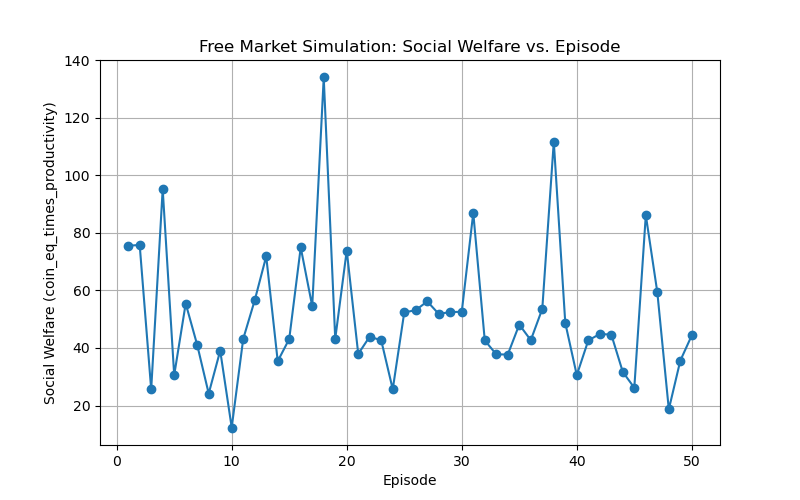
\includegraphics[width=0.6\textwidth]{fig/free_market_sw.png}
    \caption{Free Market Simulation: Social Welfare Over 50 Episodes.}
    \label{fig:free_market_sw}
\end{figure}

\subsection{Utility vs.\ Skill}

Additionally, we analyze how an agent’s skill level (10, 15, 20, 30) interacts with labor performed to yield different utility values, using an isoelastic function. The script \texttt{plot\_and\_save\_utility\_curves} scans labor from $0$ to $1000$ and plots
\[
u(\text{skill}, \text{labor}) = \frac{(\text{income}(\text{skill},\text{labor}))^{1-\eta}-1}{1-\eta} - \text{labor}.
\]
Figure below shows that higher skill yields greater maximum utility at higher labor, with diminishing returns.

\begin{figure}[H]
    \centering
    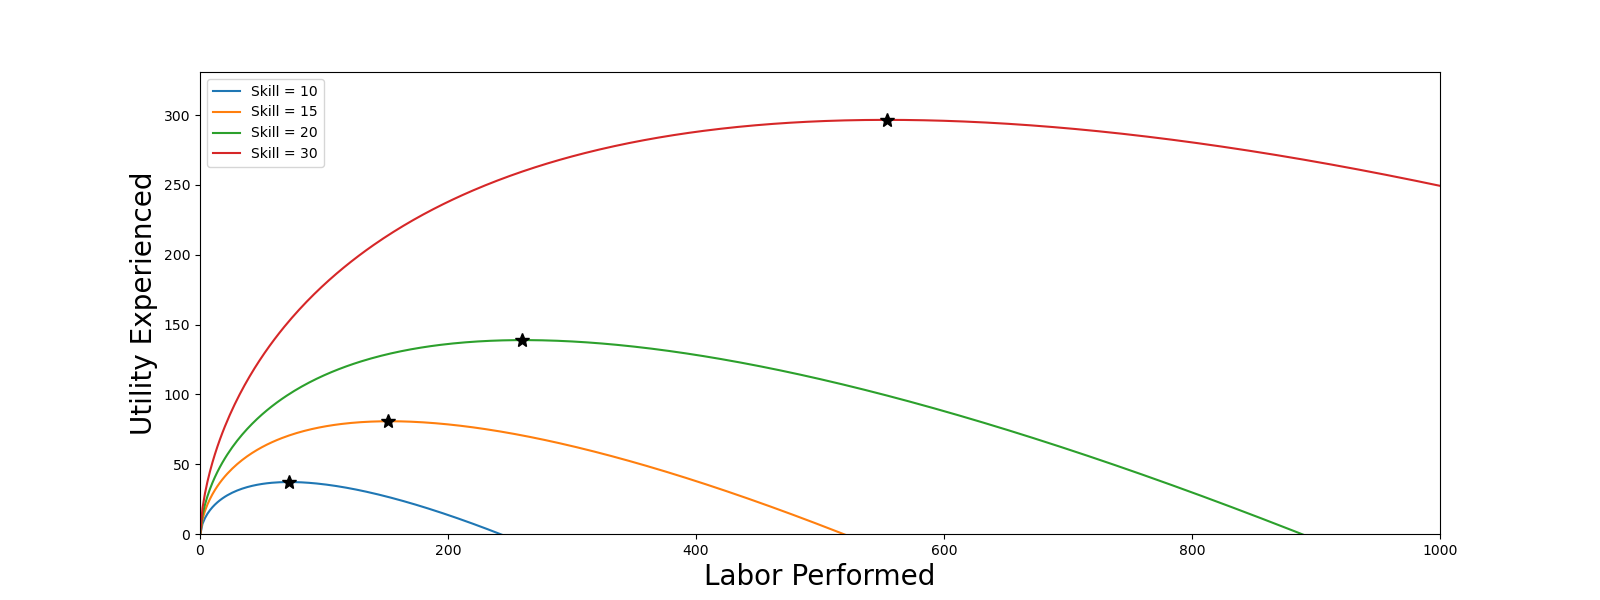
\includegraphics[width=0.6\textwidth]{fig/utility_curves_based_on_skill.png}
    \caption{Isoelastic Utility Curves for Different Skill Levels. Markers indicate the labor level that maximizes the utility at each curve.}
    \label{fig:skill_utility}
\end{figure}

\subsection{Summary of Findings}
\begin{itemize}
    \item Even in a free-market scenario, we see that higher-skill agents can outperform (e.g.\ building) if they invest more labor.
    \item Random actions are not beneficial for social welfare. This underscores the need for a trained policy or carefully guided search.
\end{itemize}
Future experiments will introduce taxes via the \texttt{PeriodicBracketTax} component and compare free-market vs.\ taxed outcomes.



\section{Citations and References}


% \bibliography{main}
% \bibliography{ref/zheng_2020_aieconomist}
% \bibliographystyle{apalike}
Zheng, S., Trott, A., Srinivasa, S., Naik, N., Gruesbeck, M., Parkes, D. C., & Socher, R. (2020). The AI Economist: Improving equality and productivity with AI-driven tax policies. arXiv. https://arxiv.org/abs/2004.13332

Schulman, J., Wolski, F., Dhariwal, P., Radford, A., & Klimov, O. (2017). Proximal Policy Optimization Algorithms. arXiv. https://arxiv.org/abs/1707.06347

\end{document}